\documentclass[a4paper,12pt]{article}

% don't forget the document class, generally : \documentclass[a4paper,12pt]{article}

\usepackage[utf8]{inputenc}
\usepackage[french]{babel}
\usepackage{graphicx}
\usepackage{gensymb}
\usepackage{amsmath}
\usepackage{float}
\usepackage{scrextend}
\usepackage{caption} 
\usepackage{siunitx}
\usepackage{enumitem}
\usepackage{amsthm}
\usepackage{fancyhdr}
\usepackage{amssymb}
\usepackage{wrapfig}
\usepackage{geometry}
\usepackage{standalone}
\usepackage{import}
\usepackage[usenames, dvipsnames]{color}

 \usepackage{biblatex} % manages bibliography and references
\addbibresource{sample.bib}


\geometry{hmargin=1in, vmargin=1in}

 \newenvironment{absolutelynopagebreak}
 {\par\nobreak\vfil\penalty0\vfilneg
 \vtop\bgroup}
 {\par\xdef\tpd{\the\prevdepth}\egroup
 \prevdepth=\tpd}
 
 \pagestyle{fancy}                        
\fancyhf{}                               
\fancyhf[HL]{Application des maths}                
\fancyhf[HR]{Géométrie euclidienne}             
\fancyhf[FC]{\thepage/\pageref{Lastpage}}
 
\newtheorem{definition}{Définition}[section]
\newtheorem{theorem}{Théorème}
\newtheorem{corollary}{Corollaire}[theorem]
\newtheorem{lemma}[theorem]{Lemme}
\newtheorem*{hyp}{Hypothèse}
\newtheorem*{concl}{Conclusion}
\newtheorem*{remark}{Remarque}

\captionsetup{format=default,labelformat=simple,labelsep=colon,
justification=justified,font={sf,small},labelfont=bf,
textfont=default} 



\begin{document}

\pagebreak
\subsection{Isométrie de deux angles opposés par le sommet}
\begin{theorem}
Deux angles opposés par le sommet sont isométriques.
\end{theorem}
\begin{proof}
Nous considérons deux droites sécantes.

 \begin{figure}[H]
    \centering
    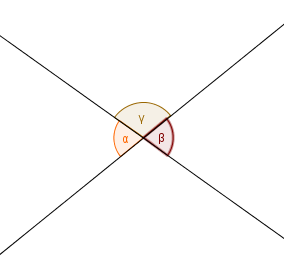
\includegraphics[scale=0.8]{theorems/oppSommet/anglesym.PNG}
\end{figure}


\begin{hyp}
     Deux droites se croisent en un point
 \end{hyp}
 \begin{concl}
     $\alpha \equiv \beta$, $\gamma$ est l'angle complémentaire de $\alpha$ et $\beta$
 \end{concl}
 Comme $\gamma$ est l'angle complémentaire de $\alpha$ et $\beta$, on peut écrire l'équation suivante:
 \begin{equation}
 \gamma + \alpha = 180\degree \rightarrow \alpha = 180\degree-\gamma
 \end{equation}
 \begin{equation}
 \gamma+ \beta = 180\degree \rightarrow \beta = 180\degree-\gamma
 \end{equation}
 Par conséquent, on sait que $\alpha \equiv \beta$.
\end{proof}

\end{document}
